\documentclass{article}
\usepackage{graphicx}
\usepackage{amssymb}
\usepackage{amsmath}
\usepackage{float}
\usepackage{hyperref}
\usepackage[margin=1in]{geometry}

\begin{document}

\title{Robotics 811 - Homework 4}
\author{Xiang Zhi Tan}
\maketitle

\section{Q1}
\subsection*{1(a)}
Fristly, we notice that the equation is a separative form of differentiation and can be separate into 
\begin{equation*}
\begin{aligned}
\frac{dy}{dx} &= \frac{2}{x^2} (1-y) \\
(1-y) dy &= \frac{2}{x^2} dx 
\end{aligned}
\end{equation*}
By applying integration to both side, we get
\begin{equation*}
\begin{aligned}
\int (1-y) dy &= \int \frac{2}{x^2} dx \\
y - \frac{1}{2}y^2 + c &= -2 x^{-1} + c
\end{aligned}
\end{equation*}
By observing the equation, we notice it has the form of a quadratic equation, we then rearrange it and put it into the form of the quadratic formula.
\begin{equation*}
\begin{aligned}
y - \frac{1}{2}y^2 + c &= -2 x^{-1} + c\\
-\frac{1}{2}y^2 + y +(2x^{-1} - c) &= 0\\
y^2 + (-2y) +(-4x^{-1} + c) &= 0\\
y &= \frac{2 \pm \sqrt{4 - 4(-4x^{-1} + c)}}{2}\\
y &= 1 \pm \frac{\sqrt{4 + 16x^{-1} - 4c}}{2}\\
y &= 1 \pm \frac{\sqrt{4}\sqrt{1 + 4x^{-1} - c}}{2}\\
y &= 1 \pm \sqrt{1 + 4x^{-1} -c}\\
y &= 1 \pm \sqrt{4x^{-1} - c}
\end{aligned}
\end{equation*}
Because we know the initial condition of $y(1) = -1$, we can plug it back into the previous equation and solve for $c$
\begin{equation*}
-1 = 1 \pm \sqrt{\frac{4}{1} - c}
\end{equation*}
Because the square root will be positive, the only way to have a negative on the lefthand side would be that the $\pm$ is a negative sign.
\begin{equation*}
\begin{aligned}
-1 &= 1 - \sqrt{4 - c}\\
2 &= \sqrt{4 - c}\\
c & = 0 
\end{aligned}
\end{equation*}
Now, we kno that the analytic solution would be the following:
\begin{equation*}
y(x) = 1 - 2 \sqrt{x^{-1}}
\end{equation*}
\subsection*{1(b)}
We impleted and used the Euler Method, following is the table with the found value and real answer from the expected value\\
\begin{center}
\begin{tabular}{|c|c|c|c|}
\hline
n & x & y & real y \\ \hline
0 & 1.000000 & -1.000000 & -1.000000 \\ \hline 
1 & 0.950000 & -1.050000 & -1.051957 \\ \hline 
2 & 0.900000 & -1.104050 & -1.108185 \\ \hline 
3 & 0.850000 & -1.162726 & -1.169305 \\ \hline 
4 & 0.800000 & -1.226723 & -1.236068 \\ \hline 
5 & 0.750000 & -1.296894 & -1.309401 \\ \hline 
6 & 0.700000 & -1.374293 & -1.390457 \\ \hline 
7 & 0.650000 & -1.460248 & -1.480695 \\ \hline 
8 & 0.600000 & -1.556452 & -1.581989 \\ \hline 
9 & 0.550000 & -1.665109 & -1.696799 \\ \hline 
10 & 0.500000 & -1.789149 & -1.828427 \\ \hline 
11 & 0.450000 & -1.932562 & -1.981424 \\ \hline 
12 & 0.400000 & -2.100956 & -2.162278 \\ \hline 
13 & 0.350000 & -2.302507 & -2.380617 \\ \hline 
14 & 0.300000 & -2.549691 & -2.651484 \\ \hline 
15 & 0.250000 & -2.862707 & -3.000000 \\ \hline 
16 & 0.200000 & -3.276924 & -3.472136 \\ \hline 
17 & 0.150000 & -3.861457 & -4.163978 \\ \hline 
18 & 0.100000 & -4.775677 & -5.324555 \\ \hline 
19 & 0.050000 & -6.507076 & -7.944272 \\ \hline 
20 & 0.000000 & -11.835382 & -Inf \\ \hline 
\end{tabular}
\end{center}
By observing the values, we notice this method is not too accurate and there are deviation in the end values.
\begin{equation*}
\end{equation*}
\subsection*{1(c)}
We implemented and used the fourth-order Runge-Kutta method. Following is the table containing the result
\begin{center}
\begin{tabular}{|c|c|c|c|}
\hline
n & x & y & real y \\ \hline
0 & 1.000000 & -1.000000 & -1.000000 \\ \hline 
1 & 0.950000 & -1.051957 & -1.051957 \\ \hline 
2 & 0.900000 & -1.108185 & -1.108185 \\ \hline 
3 & 0.850000 & -1.169305 & -1.169305 \\ \hline 
4 & 0.800000 & -1.236068 & -1.236068 \\ \hline 
5 & 0.750000 & -1.309401 & -1.309401 \\ \hline 
6 & 0.700000 & -1.390457 & -1.390457 \\ \hline 
7 & 0.650000 & -1.480695 & -1.480695 \\ \hline 
8 & 0.600000 & -1.581990 & -1.581989 \\ \hline 
9 & 0.550000 & -1.696800 & -1.696799 \\ \hline 
10 & 0.500000 & -1.828429 & -1.828427 \\ \hline 
11 & 0.450000 & -1.981426 & -1.981424 \\ \hline 
12 & 0.400000 & -2.162282 & -2.162278 \\ \hline 
13 & 0.350000 & -2.380624 & -2.380617 \\ \hline 
14 & 0.300000 & -2.651498 & -2.651484 \\ \hline 
15 & 0.250000 & -3.000033 & -3.000000 \\ \hline 
16 & 0.200000 & -3.472225 & -3.472136 \\ \hline 
17 & 0.150000 & -4.164292 & -4.163978 \\ \hline 
18 & 0.100000 & -5.326343 & -5.324555 \\ \hline 
19 & 0.050000 & -7.973392 & -7.944272 \\ \hline 
20 & 0.000000 & -183129202253624666683263156224.000000 & -Inf \\ \hline 
\end{tabular}
\end{center}
By observing the result, we observe that the values don't deviate until $n=8$. Compared to Euler methods, fourth-order Runge Kutta is more accurate.
\subsection*{1(d)}
We implemented and used the fourth-order  Adams-Bashforth. Following is the table containing the result.
\begin{center}
\begin{tabular}{|c|c|c|c|}
\hline
0 & 1.000000 & -1.000000 & -1.000000 \\ \hline 
1 & 0.950000 & -1.051952 & -1.051957 \\ \hline 
2 & 0.900000 & -1.108174 & -1.108185 \\ \hline 
3 & 0.850000 & -1.169285 & -1.169305 \\ \hline 
4 & 0.800000 & -1.236038 & -1.236068 \\ \hline 
5 & 0.750000 & -1.309357 & -1.309401 \\ \hline 
6 & 0.700000 & -1.390393 & -1.390457 \\ \hline 
7 & 0.650000 & -1.480601 & -1.480695 \\ \hline 
8 & 0.600000 & -1.581854 & -1.581989 \\ \hline 
9 & 0.550000 & -1.696602 & -1.696799 \\ \hline 
10 & 0.500000 & -1.828133 & -1.828427 \\ \hline 
11 & 0.450000 & -1.980974 & -1.981424 \\ \hline 
12 & 0.400000 & -2.161562 & -2.162278 \\ \hline 
13 & 0.350000 & -2.379424 & -2.380617 \\ \hline 
14 & 0.300000 & -2.649367 & -2.651484 \\ \hline 
15 & 0.250000 & -2.995918 & -3.000000 \\ \hline 
16 & 0.200000 & -3.463310 & -3.472136 \\ \hline 
17 & 0.150000 & -4.141388 & -4.163978 \\ \hline 
18 & 0.100000 & -5.248560 & -5.324555 \\ \hline 
19 & 0.050000 & -7.504348 & -7.944272 \\ \hline 
20 & 0.000000 & -15.471548 & -Inf \\ \hline 
\end{tabular}
\end{center}
By observing the result, we see that the fourth-order Adams-Bashforth is more accurate than Euler's method but less accurate then fourth-order Runge-Kutta method.
\section{Q2}

\subsection*{2(a)}
Firstly, we plotted the function in matlab using the \textit{contour} function on the range, $y=[-4,2]$ and $x=[-2,4]$. Following is the result of the contour plot
\begin{figure}[H]
\centering
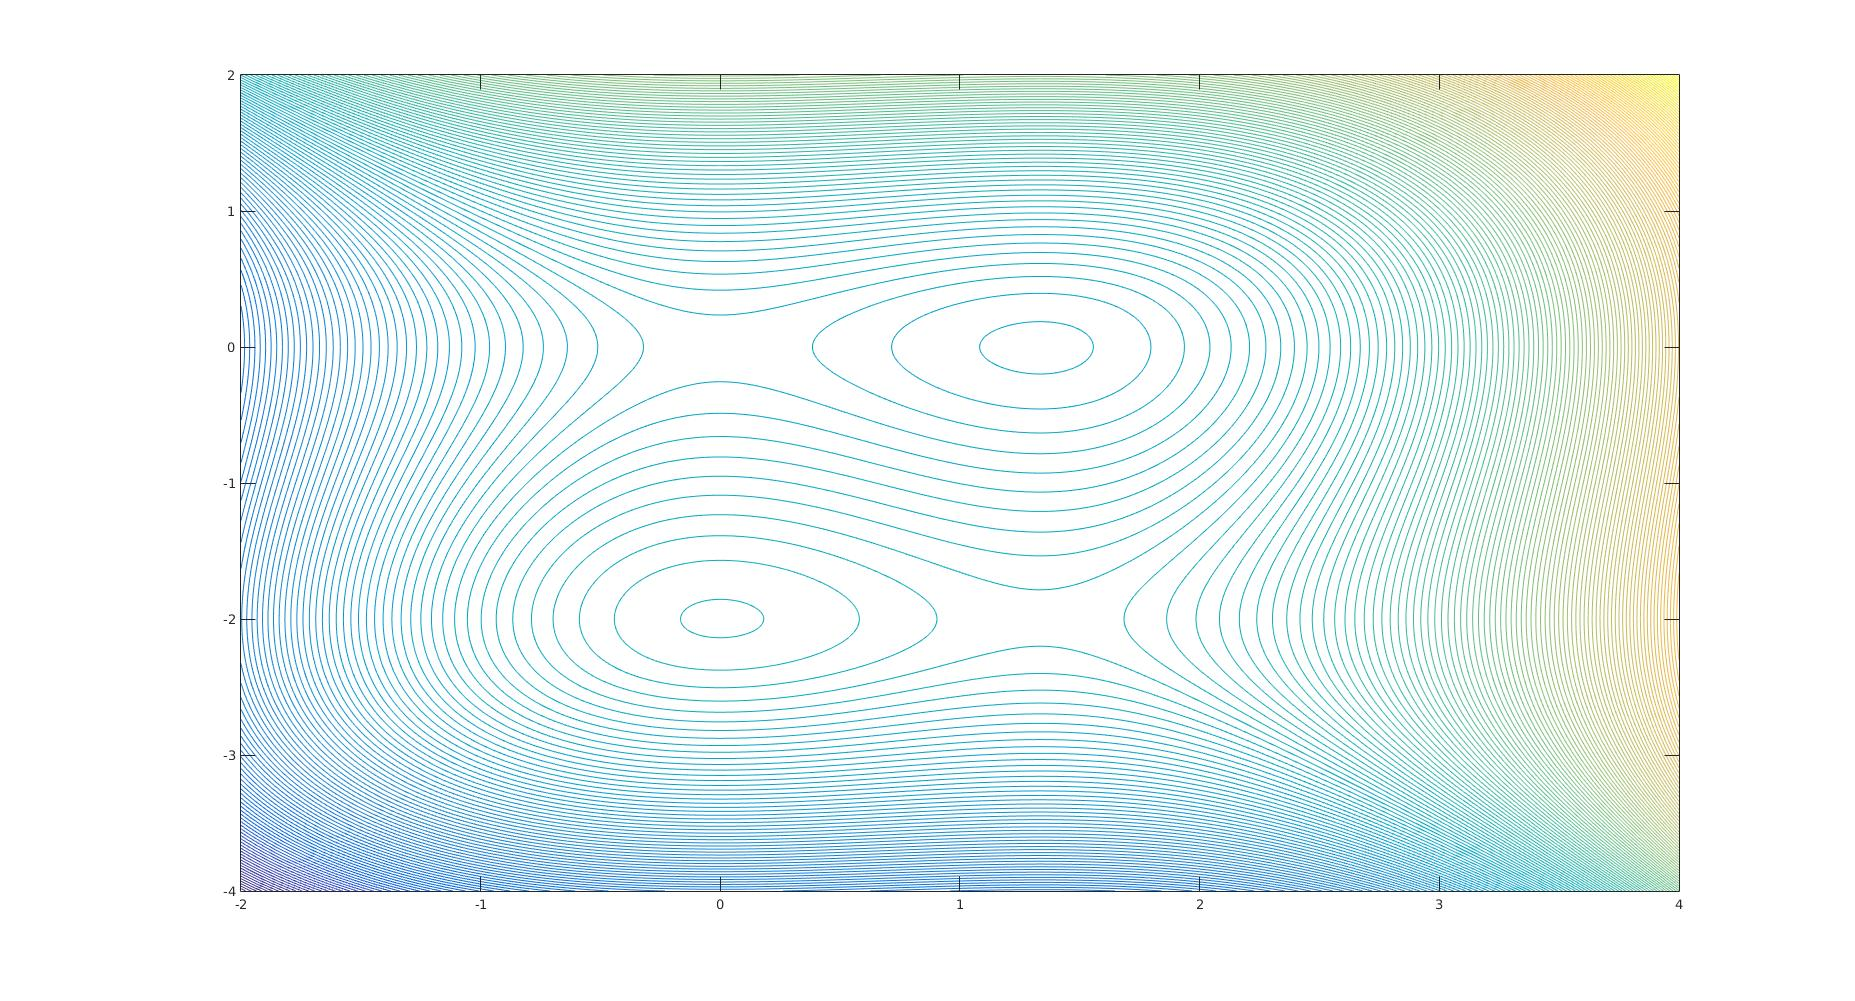
\includegraphics[width=6.5in]{figures/2a.jpg}
\caption{plot of the function $f(x,y) = x^3 + y^3 -2x^2 + 3y^2 - 8$}
\end{figure}
By examining the sketch created, we notice there are four critical points, $(0,-2),(0,0),(\frac{4}{3},-2),(\frac{4}{3},0)$.
We then measure the gradients(in the domain space) of the nearby points to determine the type of critical point. 
Following are the finding for each point:
\begin{enumerate}
\item Point$(0,-2)$\\
This is a local maxima. By measuring the gradient at 8 points around the point with a step size of $0.1$ relative to this point. we found them all to have a position gradient which means they are moving upwards towards $(0,-2)$ which means this is a local maximum\\
\item Point$(0,0)$\\
This is a saddle points. When measuring the gradient at 8 points around the point with a step size of $0.1$ relative to this point, we measured a positive gradient at the two points of $(0.1,0)$ and $(-0.1,0)$ to have a negative gradient where as the remaining 6 points to have a negative gradient. This fits the definition of a saddle point.
\item Point$(\frac{4}{3},0)$\\
This is the local minima. When measuring the gradient at the 8 points around the point with the step size of $0.1$ relative to this point, all gradients are negative, this means that the direction of all these points are towards this point meaning that this point must serve as the local minima.
\item Point$(\frac{4}{3},-2)$\\
This is a saddle points. When measuring the gradient, we found a negative gradient at point $(1.23333,-2)$ and $(1.43333,-2)$ and positive gradient at all remaining points. This shows that this must be a saddle point.
\subsection*{2(b)}
The gradient(partial derivative) of x and y can be found with the following equation:
\begin{equation*}
\begin{aligned}
\frac{\partial}{\partial x}  = x(3x - 4)\\
\frac{\partial}{\partial y}  = y(3y + 6)
\end{aligned}
\end{equation*}
Using the steepest descent algorithm, we first calculate the gradient at point $(1,-1)$. Which gives us the gradient at x, $\frac{\partial}{\partial x} = -1$ and gradient at y, $\frac{\partial}{\partial y} = -3$. Since the gradient are both non zero, we try to minimize the function $g(t) = f(x + t\vec{u})$ with u being the gradient. Minimizing the function, we found $t = \frac{1}{3}$. We update the points using the following algorithm $x^{n+1} = x^{n} - t\vec{u}$. After updating the points, we found the points to be $(\frac{4}{3},0)$ which is one of the critical points(also the local minima). The gradient at that point is also $0$, stopping the algorithm. Therefore, we need only one step to converge to the local minimum.

\end{enumerate}
\section{Q3}
\subsection*{3(a)}
First, we know that eigenvectors of Q which is a real symmetric positive definite matrix are orthogonal. This means that given two eigenvectors, $v_1$ and $v_2$ come from two distinct eigenvalues, $\lambda_1$ and $\lambda_2$. Their inner product would be 0. By grinding through the equations, we could derive the Q-orthogonal definition.
\begin{equation*}
\begin{aligned}
<v_1, v_2> &= 0\\
<\lambda_1 v_1, v2> &= 0  \mbox{  $\lambda$ is a scalar and will not change the result of the inner product}\\
<Q v_1, v_2> &= 0 \\
(Q v_1)^Tv_2 &= 0 \\
v_1^T Q^Tv_2 &= 0\\
v_1^T Q v_2 &= 0 \mbox{   the definition of Q-orthogonal}
\end{aligned}
\end{equation*}
\subsection*{3(b)}
The solution on the previous section would be sufficient as it is based on the fact that eigenvectors of Q are orthogonal to each other, which is now explicitly given.
\section{Q4}
\section{Q5}
\section{Q6}
%question 6

As we are finding the maximum area with a given parameter,$p$, we know that the objective function must be
\begin{equation*}
f(x,y) = xy
\end{equation*}
with the constraint of 
\begin{equation*}
2y + 2x - p = 0
\end{equation*}
First we construct the Lagrangian
\begin{equation*}
L(x,y,\alpha) = xy + \alpha(2y + 2x - p)
\end{equation*}
We then compute the gradient at set it to 0
\begin{equation*}
\Delta L(x,y,\alpha) = 
\begin{pmatrix}
y + 2\alpha\\
x + 2\alpha\\
2x + 2y -p \\
\end{pmatrix}
= \vec{0}
\end{equation*}
We are now given 3 equations
\begin{equation}\label{e1}
y = 2\alpha
\end{equation}
\begin{equation}\label{e2}
x = 2\alpha
\end{equation}
\begin{equation}
\begin{aligned}\label{e3}
2x &= -2y + p \\
x = \frac{-2y + p}{2}
\end{aligned}
\end{equation}
Insert \ref{e3} into \ref{e2}, we get
\begin{equation}\label{e4}
2 \alpha = \frac{-2y + p}{2}
\end{equation}
Then, insert \ref{e4} into \ref{e1}, we can solve $y$
\begin{equation}\label{e5}
\begin{aligned}
y &= \frac{-2y + p}{2}\\
2y &= -2y + p\\
y = \frac{p}{4}
\end{aligned}
\end{equation}
We then insert \ref{e5} back into \ref{e2} and we solve $x$
\begin{equation}
x = \frac{p}{4}
\end{equation}
We have now found the critical points in the equation, where $x = \frac{p}{4}$ and $y=\frac{p}{4}$. Notice that $x = y$. To show that we are achieving the maximum, we need to verify the second order sufficiency where we need to show the following matrix
\begin{equation}
L(x^*) = \Delta^2f(x*) + \alpha^T\Delta^2h(x^*)
\end{equation}
is negative semi-definate on $m$ which is $m = {y | \Delta h (x^*) y = 0}$. First we solve the partial derivatives for $f(x)$ and $h(x)$
\begin{equation*}
\begin{aligned}
\frac{\partial}{\partial^2 x} &= 0\\
\frac{\partial}{\partial^2 y} &= 0\\
\frac{\partial}{\partial xy} &= 1\\
\frac{\partial}{\partial yx} &= 1\\
\Delta^2 h &= 0\\
\end{aligned}
\end{equation*}
We have solved $L(x^*)$
\begin{equation*}
L(x^*) = 
\begin{pmatrix}
0 &1\\
1 &0\\
\end{pmatrix}
\end{equation*}
We then check where the matrix is positive semi-definite or negative semi-definite by choosing a vector from the subspace $M$ and apply $y^TLy$.
\begin{equation}
\begin{aligned}
\Delta h(x) &= [2 2]\\
[2 2]y &= 0\\
\begin{pmatrix}
y_1\\
y_2 \\
\end{pmatrix}
& = 
\begin{pmatrix}
-1 \\
1 \\
\end{pmatrix}
\end{aligned}
\end{equation} 
\begin{equation}
\begin{pmatrix}
-1 & 1 
\end{pmatrix}
\begin{pmatrix}
0 & 1 \\
1 & 0\\
\end{pmatrix}
\begin{pmatrix}
-1 \\
1
\end{pmatrix}
= -2
\end{equation}
This shows the matrix is negative semi-definite and therefore, $x^*$ must be the maximum of $f$.

\section{Q7}
\subsection*{7(a)}
We can first rearrange the constraints 2 and 3 into the following form by moving elements on the right handside to the left and multiplying constraints 2 by $-1$.
\begin{equation*}
\begin{aligned}
- w^Tx_i - b + 1 - \xi_i &\leq 0\\ \mbox{ if } y_i = 1
w^Tx_i + b + 1 - \xi_i &\leq 0\\ \mbox{ if } y_i = -1
\end{aligned} 
\end{equation*}
Through observing the inequalities, we notice that the only difference is the element $w^Tx_i$ which has a different sign that could be change by the values of $y_i$. This allows us to combine both inequalities into the following constraint.
\begin{equation*}
- y_i(w^Tx_i + b) + 1 - \xi_i \leq = 0
\end{equation*}

\subsection*{7(b)}
The Lagrangian for our optimization problem is as following:
\begin{equation*}
L ([w\;0\;\xi]^T, \alpha, \beta) = \frac{1}{2}||w||^2 + C \sum_{i=1}^l \xi_i + \sum_{i=1}^l \alpha_ig_i([w\;b\;\xi]^T) - \sum_{i=1}^l \beta_i \xi_i
\end{equation*}

\subsection*{7(c)}
Following is the steps to minimize the Lagrangian which is ther primal form of the SVM. Here's the original Lagrangian.
\begin{equation}\label{ori-l}
L ([w\;0\;\xi]^T, \alpha, \beta) = \frac{1}{2}||w||^2 + C \sum_{i=1}^l \xi_i + \sum_{i=1}^l \alpha_i(- y_i(w^Tx_i + b) + 1 - \xi_i) - \sum_{i=1}^l \beta_i \xi_i
\end{equation}
First we, find the partial of $w$,$b$ and $\xi_i$. Following are the partials follow by setting them to 0.\\
Finding partial of $w$
\begin{equation}\label{wpartial}
\begin{aligned}
\frac{\partial}{\partial w} &= \frac{2}{2} w - \sum_{i=1}^l(\alpha_i y_i x_i) = 0\\
w &= \sum_{i=1}^l(\alpha_i y_i x_i)
\end{aligned}
\end{equation}
Finding the partial of $b$.
\begin{equation}\label{bpartial}
\begin{aligned}
\frac{\partial}{\partial b} &= -\sum_{i=1}^l(\alpha_i y_i) = 0\\
\sum_{i=1}^l(\alpha_i y_i) &= 0\\
\end{aligned}
\end{equation}
Finding the partial of $xi_i$.
\begin{equation}\label{xipartial}
\begin{aligned}
\frac{\partial}{\partial \xi_i} &= C - \sum_{i=1}^l(\alpha_i) - \sum_{i=1}^l(\beta_i) = 0\\
C &= \sum_{i=1}^l(\alpha_i) + \sum_{i=1}^l(\beta_i)
\end{aligned}
\end{equation}\tabularnewline
Now we insert equations \ref{wpartial}, \ref{xipartial} in equation \ref{ori-l}.
\begin{equation}
\begin{aligned}
L &= \frac{1}{2}(\sum_{i=1}^l(\alpha_i y_i x_i))^2 + (\sum_{i=1}^l(\alpha_i) + \sum_{i=1}^l(\beta_i))\sum_{i=1}^l \xi_i + \sum_{i=1}^l \alpha_i(- y_i((\sum_{j=1}^l(\alpha_j y_j x_j))x_i + b) + 1 - \xi_i) - \sum_{i=1}^l \beta_i \xi_i\\
L &= \frac{1}{2}(\sum_{i=1}^l\sum_{j=1}^l(\alpha_i \alpha_j y_i y_j x_j^T x_i)) + \sum_{i=1}^l(\alpha_i \xi_i) + \sum_{i=1}^l(\beta_i \xi_i) + \sum_{i=1}^l(\alpha_i \alpha_j y_i y_j x_j^T x_i))\\
&- b \sum_{i=1}^l(\alpha_i y_i) + \sum_{i=1}^l(\alpha_i) - \sum_{i=1}^l(\alpha_i \xi_i) - \sum_{i=1}^l \beta_i \xi_i\\
L &= \sum_{i=1}^l(\alpha_i) - \frac{1}{2}(\sum_{i=1}^l\sum_{j=1}^l(\alpha_i \alpha_j y_i y_j x_j^T x_i)) - b \sum_{i=1}^l(\alpha_i y_i)\\
\end{aligned}
\end{equation}
By applying equation \ref{bpartial} in the previous equation, we can derive the final form
\begin{equation}\label{final-eq}
L^*(\alpha) = \sum_{i=1}^l(\alpha_i) - \frac{1}{2}(\sum_{i=1}^l\sum_{j=1}^l(\alpha_i \alpha_j y_i y_j x_j^T x_i))\\
\end{equation}

\subsection*{7(d)}
As we want to write the equation in terms of $H$ and $f$ such that $L^*(\alpha) = \frac{1}{2} \alpha^TH\alpha + f^T\alpha$. By looking at equation \ref{final-eq}, we see a similar structure between them. For the first part $\frac{1}{2} \alpha^TH\alpha $
\begin{equation*}
\begin{aligned}
\frac{1}{2}\alpha^TH\alpha &= \frac{1}{2}(\sum_{i=1}^l\sum_{j=1}^l(\alpha_i \alpha_j y_i y_j x_j^T x_i))\\
H &= (\sum_{i=1}^l\sum_{j=1}^l(y_i y_j x_j^T x_i))
\end{aligned}
\end{equation*}
For second part $f^T\alpha$
\begin{equation*}
\begin{aligned}
f^T\alpha &= \sum_{i=1}^l(\alpha_i)\\
f^T &= [1,1,.....1]
\end{aligned}
\end{equation*}

\end{document}